% =====================================================================
%  Predicting Bagrut Success — Final Report (Data Science Laboratory)
%  Authors: Yousef Shihade & Shada Esawi
%  University of Haifa
%
%  Build:  pdflatex main.tex   (run twice for cross-references)
%  This file holds the preamble + \input calls only; prose lives in sections/.
% =====================================================================
\documentclass[11pt]{article}

\usepackage[a4paper,margin=1in]{geometry}
\usepackage[T1]{fontenc}
\usepackage{lmodern}
\usepackage{microtype}          % subtle spacing improvements for tight page budgets
\usepackage{graphicx}
\usepackage{array}              % >{...} column modifiers (ragged-right fixed-width cells)
\usepackage{booktabs}           % clean tables (\toprule/\midrule/\bottomrule)
\usepackage{caption}
\usepackage{subcaption}
\usepackage{float}
\usepackage{amsmath}
\usepackage{siunitx}
\usepackage{xcolor}
\usepackage[hidelinks]{hyperref}

\graphicspath{{figures/}}

% --- compact, readable defaults for an 8-page report -----------------
\captionsetup{font=small,labelfont=bf,skip=4pt}
\setlength{\parskip}{0.30em}
\setlength{\parindent}{0pt}
\definecolor{linknavy}{HTML}{1b2a4a}
\hypersetup{
  colorlinks=true,
  allcolors=linknavy,
  pdftitle={Predicting Bagrut Success: Municipal Socioeconomics and School-Level Institutional Resources},
  pdfauthor={Yousef Shihade, Shada Esawi},
  pdfsubject={School-level prediction of Bagrut achievement and advanced-track participation},
  pdfkeywords={Bagrut, education, socioeconomic status, machine learning, SHAP, nested cross-validation}
}

% Repository URL, used in the Introduction's Code Availability line.
\newcommand{\repourl}{https://github.com/Yousef-Shihade/predicting-bagrut-success}

% =====================================================================
\begin{document}

% --- compact title block (not a full title page — conserves the page budget)
\begin{center}
    {\LARGE\bfseries Predicting Bagrut Success}\\[16pt]
    {\large Yousef Shihade \quad Shada Esawi}\\[14pt]
    University of Haifa \,\textbullet\, Data Science Lab -- Final Project 2026\\[10pt]
    \rule{\textwidth}{0.4pt}
\end{center}

\section{Introduction}

Every year Israeli high-school students sit the \emph{Bagrut}, the national
matriculation examinations that gate university admission. A long-standing
question in educational policy is how much a student's outcome is fixed by the
socioeconomic status of the \emph{municipality} their school sits in, versus what
the \emph{school itself} does with its resources. This project answers that
question with a reproducible, cross-validated machine-learning pipeline.

\textbf{Main question.} Can municipal socioeconomic status and school-level
institutional resources, \emph{combined}, meaningfully predict Israeli
high-school Bagrut achievement and advanced-track participation? \textbf{Secondary
questions.} (A)~Which subject (Mathematics or English) is more \emph{resilient}
to socioeconomic and institutional disparity, and do schools exist that
outperform their peers despite limited resources? (B)~Which specific school-level
factors (budget allocation, class size, sector, or supervision type) most
strongly predict outcomes, \emph{independent} of municipal wealth?

We model four school-level targets: the average Bagrut grade and the advanced
(5-unit) participation rate, each for Mathematics and English. A municipal score
cannot capture what happens inside a specific school, and separating the two is
what makes the policy question answerable.

\textbf{Revisions since the interim stage.} The study began as a municipal-only
design. Following review we added the Ministry's school-level dataset and rebuilt
the pipeline from ingestion onward. Later revisions introduced cross-validation
grouped by school, per-target feature selection, explicit handling of
privacy-suppressed grades, a municipal-versus-school ablation, and a nested
protocol in which feature selection and tuning run inside training folds only.

\textbf{Code availability.} All data-processing and modelling code, with
per-stage documentation, is openly available at \href{\repourl}{\repourl}. Every
figure and number below traces to a file in that repository.

\section{Data Description and Collection}

This study integrates \textbf{three} independent, publicly available sources,
each describing Israeli high schools from a different angle. \textbf{(1)~Bagrut
exam records} (2013--2016), released under the Israeli Freedom of Information Law
and mirrored on Kaggle, give per-subject results for each school and year.
\textbf{(2)~The Central Bureau of Statistics (CBS) socioeconomic index}
rates every locality on a 1--10 cluster capturing municipal wealth, education,
and employment. \textbf{(3)~The Ministry of Education's school budget and
institutional report} provides per-institution funding, staffing, class size,
sector, and supervision type. Source~1 supplies the \emph{outcomes}, source~2 the
\emph{municipal} environment, and source~3 lets us look \emph{inside} the school
itself. The unit of analysis is the \emph{school-year}, not the student.

\textbf{Structure and storage.} The Bagrut file is a UTF-8 CSV. The CBS and
Ministry files are Excel workbooks with awkward layouts (a header offset, Hebrew
column names, and a malformed style block requiring a lenient reader). Each
source is ingested by a dedicated loader and cached as a clean CSV
(Table~\ref{tab:datasets}).

\begin{table}[ht]
\centering
\small
\renewcommand{\arraystretch}{1.35}
\caption{The three integrated data sources: one supplies the outcomes, one the
municipal context, and one the school's own institutional profile. This split is
what lets the study separate ``where a school is'' from ``what a school does''.}
\label{tab:datasets}
\begin{tabular}{@{}>{\raggedright\arraybackslash}p{2.9cm}>{\raggedright\arraybackslash}p{2.5cm}rr>{\raggedright\arraybackslash}p{2.9cm}l@{}}
\toprule
\textbf{Dataset} & \textbf{Source} & \textbf{Rows} & \textbf{Cols} & \textbf{Grain (key)} & \textbf{Coverage} \\
\midrule
Bagrut exam records & Israeli FOI (Kaggle) & 69,638 & 9 & subject cell (1,063 schools, 315 cities) & 2013--2016 \\
CBS socioeconomic index & Israel CBS & 1,208 & 7 & locality (cluster 1--10) & 2015 index \\
Ministry budget \& institution report & Israel Min.\ of Education & 4,718 & 26 & school (\texttt{semel}) & 2014/15 snapshot \\
\bottomrule
\end{tabular}
\end{table}

\textbf{Linking the sources.} The tables are joined on \emph{two different keys},
because \texttt{semel} is not shared consistently: in the Bagrut file it is a
\emph{school} code, in the CBS file a \emph{locality} code, giving zero overlap.
We therefore (i)~join Bagrut to CBS on a \emph{normalised Hebrew locality name}
through a four-stage cascade
(exact~$\rightarrow$~structural~$\rightarrow$~hand-verified crosswalk~$\rightarrow$~conservative
fuzzy match), integrating \textbf{99.44\%} of records, and (ii)~join Bagrut to
the Ministry report directly on \texttt{semel} (a shared \emph{school} code),
integrating \textbf{99.68\%}. A left join can multiply rows when the right-hand
key repeats, so each lookup table is de-duplicated on its join key first. This
matters because the normalised locality name is not unique in the CBS file. Row
preservation was verified rather than assumed: the merged table has exactly
\textbf{69,638} rows, matching the Bagrut input, and \textbf{98.7\%} of records
carry a complete profile from all three sources.

\textbf{Biases and challenges.} Three were material. The key incompatibility
above is resolved by the name cascade rather than a fragile single-pass match.
The Ministry report is a single-year (2014/15) snapshot broadcast across all four
Bagrut years, a documented limitation that assumes school resourcing is
reasonably stable over 2013--2016. Finally, the unmatched 0.56\% of records
(boarding and regional schools with no single home municipality) are
\emph{flagged, not forced}, avoiding an invented socioeconomic value.

\section{Data Cleaning and Preprocessing}

Cleaning addressed four concerns: the missing target, predictor imputation,
outliers, and encoding.

\textbf{The missing target is not missing at random.} 21.4\% of Bagrut grade
values are absent, but the absence is structured: suppressed cells have a median
of 7 test takers against 28 where the grade is present. This is the Ministry
protecting the privacy of small cohorts, not random loss. We therefore
\emph{never impute the target}. School-level grades are aggregated over observed
cells only, so no outcome value is invented.

\textbf{Imputation is measured, not assumed.} Rather than assuming multivariate
imputation by chained equations (MICE) recovers missing predictor values well, we
test it directly: we hide 8\% of a fully observed feature (the CBS socioeconomic
score), reconstruct it with MICE, and score the reconstruction against the
withheld truth over 25 independent masks. MICE beats a median baseline on all 25 runs, but the
margin depends on what else is available. With the municipal \texttt{cluster} in
the predictor set MICE reaches $R^2 = 0.954 \pm 0.006$, a number that flatters
the method because \texttt{cluster} is a discretisation of the same index
($r = 0.97$). Withholding that near-duplicate and the outcome columns, MICE still
reaches $R^2 = 0.331 \pm 0.056$ (RMSE $0.755$) while the median baseline never
rises above zero, and it wins all 25 masks in every predictor set tested. MICE
reconstructs each gap from the other observed columns, whereas the median returns
one value everywhere and cannot track variation at all. Per-variant results are
in the repository.

\textbf{Modelling itself uses complete cases.} The masking study is a diagnostic.
Imputed values are \emph{not} carried into the modelling table. Rows missing any
numeric predictor are dropped, costing 9.0\% to 12.5\% of the target-present rows
depending on the outcome, leaving 2,963 to 3,226 school-years per target. Missing
categorical values enter as an all-zero indicator pattern.

\textbf{Outliers are flagged, and kept in the primary analysis.} Two
complementary detectors, Isolation Forest (global anomalies) and the Local
Outlier Factor (local-density anomalies), were run on a nine-feature space. They
agree on only 49 records (Jaccard $0.17$), confirming they capture genuinely
different notions of ``anomalous''. That feature space includes outcome
variables, so excluding the flagged rows would condition the evaluation sample on
the target and could quietly remove legitimate high or low performers. The
primary results therefore retain every valid school. Repeating the evaluation
with the 49 records dropped changes mean $R^2$ by $+0.001$, with per-target
shifts between $-0.023$ and $+0.013$, well inside the fold-to-fold standard
deviation. The choice is immaterial to the findings.

\textbf{Encoding and scaling.} Categorical attributes (sector, supervision,
district, legal status, education stage, locality type) are one-hot encoded, with
Hebrew values mapped to English first for readable outputs. The exam
\texttt{year} is encoded as four independent periods rather than a numeric trend,
since with only four years there is no basis to assume an equal step between
them. Linear models are standardised inside the cross-validation folds, never on
the full dataset, so no test-fold information leaks into the scaling. Trees need
no scaling.

\section{Machine Learning Models}
\label{sec:models}

The task is \textbf{regression, not classification}. Four continuous
school-level outcomes are predicted, each on its own: two grade averages on a
0--100 scale (\texttt{math\_avg\_grade}, \texttt{english\_avg\_grade}) and two
advanced-track (5-unit) participation rates on a 0--1 scale
(\texttt{math\_5unit\_participation}, \texttt{english\_5unit\_participation}).

\textbf{Four model families compete on equal terms.} Rather than commit to one
algorithm, we span the useful complexity range from a regularised linear fit to
modern boosted trees (Table~\ref{tab:models}). Every family is tuned within the
same inner folds using a predefined model-specific search space and up to 25
candidate configurations. Ridge's seven regularisation values are evaluated
exhaustively. An earlier version of this study tuned only the boosted-tree model
and left the others at defaults, which makes any conclusion about a winner an
artefact of unequal effort rather than a property of the data.

\begin{table}[H]
\centering
\footnotesize
\renewcommand{\arraystretch}{1.15}
\caption{The four competing model families. All are tuned under the same nested
protocol using model-specific hyperparameter spaces.}
\label{tab:models}
\begin{tabular}{@{}>{\raggedright\arraybackslash}p{2.2cm}>{\raggedright\arraybackslash}p{1.9cm}>{\raggedright\arraybackslash}p{9.7cm}@{}}
\toprule
\textbf{Model} & \textbf{Family} & \textbf{Why it fits this problem} \\
\midrule
Ridge & Linear (L2) & Stable linear baseline the trees must beat. L2 shrinkage handles the many one-hot dummies well. \\
SGD linear & Linear (SGD) & Second linear fit by stochastic gradient descent, a check that the linear result is not a solver artefact. \\
Random Forest & Bagged trees & Captures non-linearities and interactions without scaling. Bagging resists overfitting. \\
Hist\-Gradient\-Boosting & Boosted trees & Efficient boosted-tree model capturing nonlinear relationships and feature interactions in encoded tabular data. \\
\bottomrule
\end{tabular}
\end{table}

\textbf{Nested cross-validation keeps the evaluation honest.} Two kinds of
leakage matter. Structurally, each school contributes up to four year-rows
(2013--2016), so folds are formed by school using GroupKFold(\texttt{semel}).
More subtly, if feature selection or tuning sees the whole dataset then the
evaluation folds have already influenced the model and scores become optimistic.
We therefore \emph{nest}: an outer GroupKFold supplies untouched evaluation
folds, and within each outer \emph{training} fold only we run VIF pruning, Boruta
selection, and an inner GroupKFold search. Every number in
Table~\ref{tab:leaderboard} is an outer-fold result, reported as a mean and
standard deviation across folds.

\begin{table}[H]
\centering
\footnotesize
\renewcommand{\arraystretch}{1.3}
\caption{Comparative model performance: outer-fold $R^2$ (mean $\pm$ standard
deviation over five folds), each family tuned under the same protocol. Random
Forest leads on every target, though the families sit within roughly one
standard deviation of each other on the grade outcomes.}
\label{tab:leaderboard}
\begin{tabular}{@{}>{\raggedright\arraybackslash}p{4.5cm}cccc@{}}
\toprule
\textbf{Target} & \textbf{Ridge} & \textbf{SGD} & \textbf{Rand.\ Forest} & \textbf{HistGB} \\
\midrule
\texttt{math\_avg\_grade}              & $0.405\!\pm\!0.066$ & $0.402\!\pm\!0.058$ & $\mathbf{0.420\!\pm\!0.050}$ & $0.414\!\pm\!0.054$ \\
\texttt{english\_avg\_grade}           & $0.410\!\pm\!0.045$ & $0.410\!\pm\!0.043$ & $\mathbf{0.452\!\pm\!0.042}$ & $0.441\!\pm\!0.043$ \\
\texttt{math\_5unit\_participation}    & $0.323\!\pm\!0.043$ & $0.323\!\pm\!0.041$ & $\mathbf{0.395\!\pm\!0.037}$ & $0.378\!\pm\!0.030$ \\
\texttt{english\_5unit\_participation} & $0.502\!\pm\!0.036$ & $0.504\!\pm\!0.037$ & $\mathbf{0.557\!\pm\!0.053}$ & $0.539\!\pm\!0.064$ \\
\bottomrule
\end{tabular}
\end{table}

Random Forest is selected for every target, though two observations temper the
ranking. On the grade outcomes all four families lie within about one standard
deviation of one another, so the algorithm matters far less than the features.
The trees separate more clearly on participation, where the outcome is bounded
and the relationships less linear. Feature selection was stable across folds:
11--12 features for the Math targets and 13--15 for English.

\section{Feature Selection Methods}
\label{sec:features}

Feature selection runs in two stages: first remove predictors that are redundant
with each other, then keep only those that carry real signal for the outcome.

\textbf{Removing collinearity by iterative VIF pruning.} From 15 numeric
candidates, instead of dropping every feature above the variance-inflation
threshold (VIF $>5$) at once, we drop the single worst offender and recompute
until every survivor clears it, because inflation is usually shared between a
pair. Several features look collinear at first (the teaching-budget ratio at
VIF $\approx 77$, individual-instruction hours at $\approx 58$, \texttt{cluster}
at $\approx 20$), but most of that collapses once the true culprit goes. Only
three drops are needed: two redundant budget ratios and the raw
\texttt{index\_value}, which duplicates the \texttt{cluster} built from it.
\texttt{cluster} itself survives once \texttt{index\_value} is gone, leaving
twelve numeric features.

\textbf{Keeping relevance by Boruta, per target.} On those 12 survivors plus
seven one-hot categorical blocks (sector, supervision, district, legal status,
education stage, locality type, year), totalling 49 encoded columns, Boruta runs
separately for each target. Using a 200-tree random forest it compares every real feature
against randomly shuffled shadow copies over up to 100 iterations, retaining one
only when its importance repeatedly exceeds the 90th percentile of the shadow
importances. A predictor survives only if its signal is dependably stronger than
noise.

The result is a \textbf{nine-feature core} confirmed for all four targets:
locality population, the nurture index, average class size, school size, and five
per-student budget ratios (tuition, perimeter, projects, purchases, transport).
Each target adds its own on top (Table~\ref{tab:boruta}). Notably
\texttt{cluster} is \emph{not} in that core: municipal status is confirmed for
three targets but rejected outright for English average grade. Five core features
are budget lines, and every target confirms at least one sector, supervision, or
district attribute, a first sign that school-level structure carries signal the
municipal cluster does not. No \texttt{year} dummy is confirmed anywhere, which
says nothing about the shape of a temporal trend but does mean no single exam
year carried enough independent signal to be retained.

Feature selection is repeated independently inside every outer training fold for
performance evaluation. Table~\ref{tab:boruta} reports the final descriptive
Boruta selection obtained by refitting on all available modelling rows after
evaluation. This final fit is used for interpretation and SHAP analysis, not for
estimating predictive performance.

\begin{table}[H]
\centering
\footnotesize
\renewcommand{\arraystretch}{1.3}
\caption{Boruta selections per target: the shared nine-feature core plus each
target's own confirmed additions. Extras are genuinely target-specific, not
cumulative. Municipal \texttt{cluster} appears as an addition for three targets
and is rejected for \texttt{english\_avg\_grade}.}
\label{tab:boruta}
\begin{tabular}{@{}>{\raggedright\arraybackslash}p{3.4cm}>{\raggedright\arraybackslash}p{8.6cm}r@{}}
\toprule
\textbf{Target} & \textbf{Additions beyond the nine-feature core} & \textbf{Total} \\
\midrule
Math grade      & \texttt{cluster}, \texttt{supervision\_Haredi} & 11 \\
Math 5-unit     & \texttt{cluster}, \texttt{district\_North}, \texttt{sector\_Jewish} & 12 \\
English 5-unit  & \texttt{cluster}, \texttt{private\_\allowbreak hours\_\allowbreak per\_student}, \texttt{sector\_Jewish}, \texttt{supervision\_Haredi} & 13 \\
English grade   & \texttt{district\_North}, \texttt{private\_\allowbreak hours\_\allowbreak per\_student}, \texttt{special\_\allowbreak ed\_share}, \texttt{sector\_Bedouin} & 13 \\
\bottomrule
\end{tabular}
\end{table}

\section{Performance Evaluation and Cross-Validation}
\label{sec:evaluation}

\textbf{Three metrics, each guarding a different failure.} Every model is scored
on three complementary regression metrics rather than one. $R^2$ reports the
share of outcome variance explained, which is scale-free and so comparable across
the four targets. RMSE gives the typical error in the target's own units and
penalises large misses heavily. MAE gives the plain average absolute error, which
is robust to a few extreme cases. Reporting all three means no single number can
flatter a model: a low RMSE paired with a poor $R^2$, for instance, would expose
a model that looks precise only because the outcome barely varies. Because the
task is regression, class imbalance does not apply, but the target distributions
were still inspected. Both participation outcomes are right-skewed, advanced
Math especially, and that skew reappears in the residuals below.

\textbf{Errors in interpretable units.} For the selected model the grade targets
carry an MAE of 4.11 points (Math) and 3.45 (English) on the 0--100 scale, with
RMSE 5.37 and 4.53. The participation targets carry an MAE of 5.8 and 13.1
percentage points, with RMSE 8.5 and 17.8. The English participation error is the
largest in absolute terms, consistent with that outcome having the widest spread
across schools.

\textbf{Residual diagnostics.} Figure~\ref{fig:residuals} shows the distribution
of the nested out-of-fold residual (actual minus predicted) per target. Because
these predictions come from outer folds never used for selection or tuning, the
diagnostic matches the protocol behind Table~\ref{tab:leaderboard}. Every mean
residual is within $0.03$ of zero, so there is no material \emph{global} bias,
though this does not rule out subgroup bias or calibration error at the extremes.
The grade models are near-symmetric. The participation models are centred on zero
but mildly right-skewed, because the outcome is itself bounded and right-skewed:
the model slightly over-predicts the many low-participation schools and
under-predicts the rare high ones. No panel shows a second peak or heavy
structured tail, though residual-versus-fitted and subgroup diagnostics would be
needed before attributing the remainder to irreducible noise.

\begin{figure}[H]
\centering
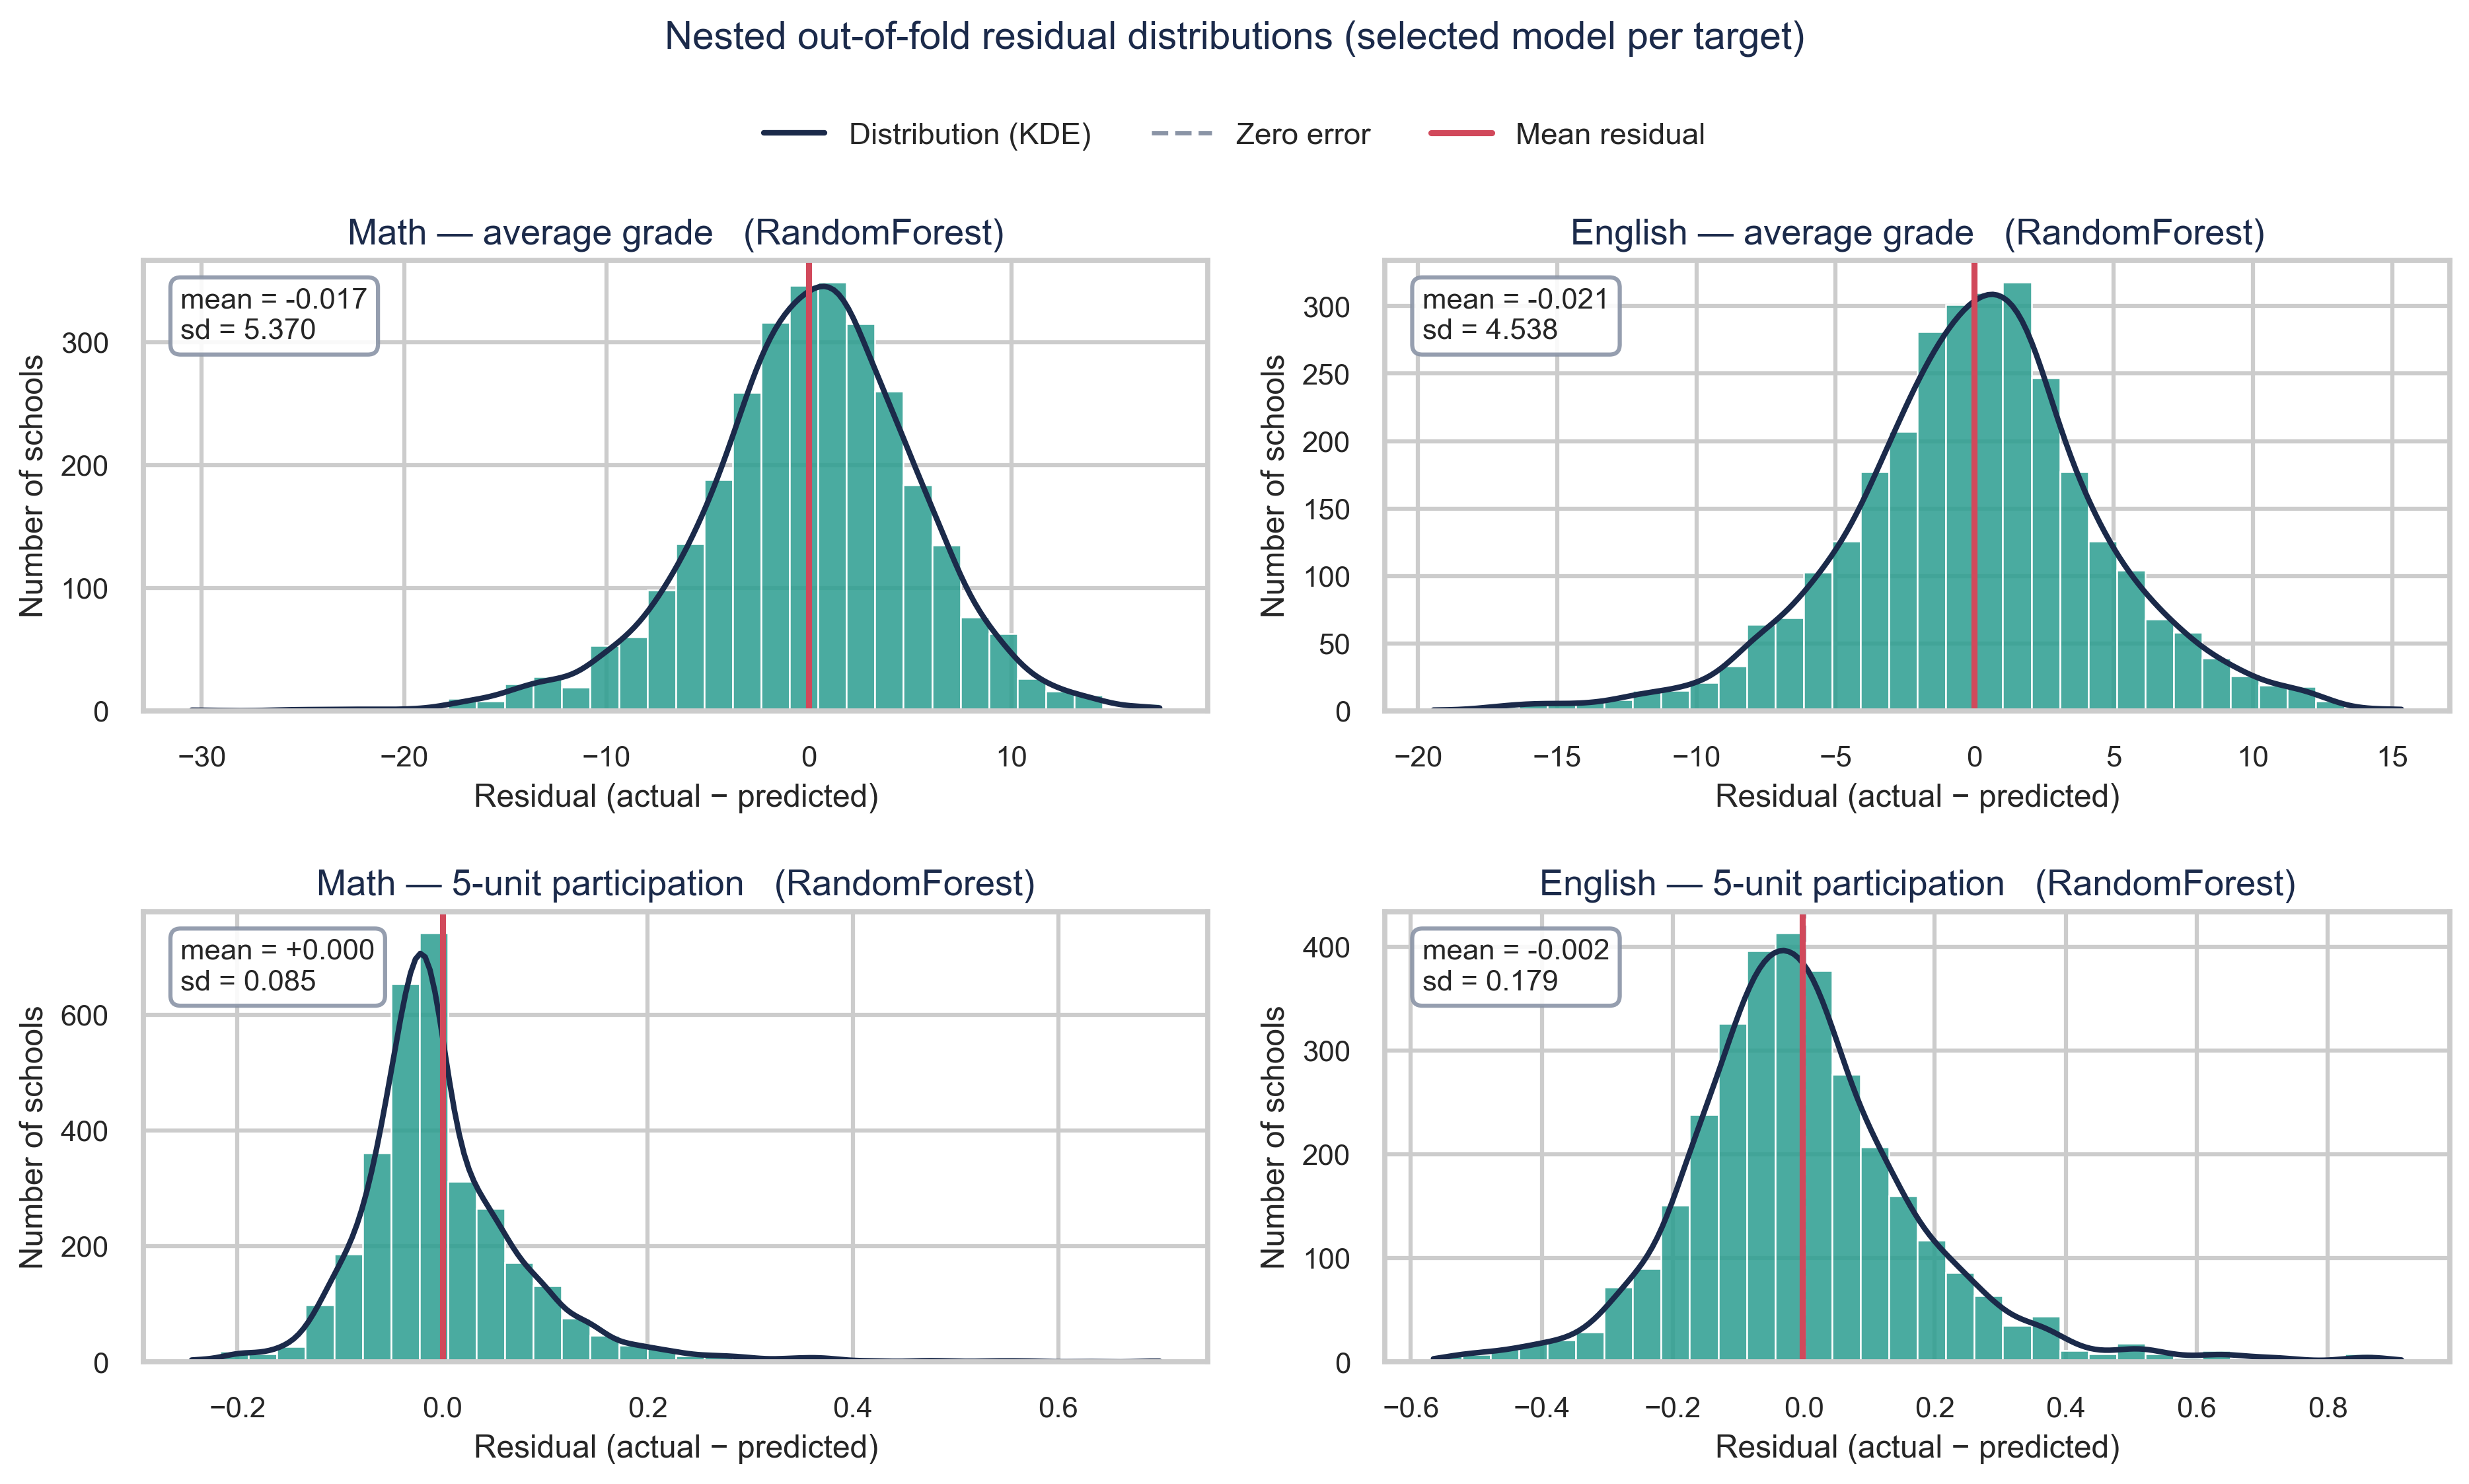
\includegraphics[width=0.78\linewidth]{section6/residuals_nested.png}
\caption{Nested out-of-fold residual distributions for the selected model, with
each panel's mean and standard deviation annotated. The coral mean line sits on
the grey zero line in all four panels.}
\label{fig:residuals}
\end{figure}

\section{Feature Analysis and Importance}
\label{sec:importance}

Two analyses answer the main research question. SHAP attributes each
prediction to individual features, and a controlled ablation measures what the
school-level data adds over municipal socioeconomics alone.

\textbf{What the models actually rely on.} Figure~\ref{fig:shap} ranks the nine
features confirmed for all four targets, plus municipal \texttt{cluster} for
comparison, by mean absolute SHAP value as a share of each target's total so the
outcomes sit on one scale. These values come from a RandomForest refitted on all
rows using the same Boruta-selected features per target, matching the family
Table~\ref{tab:leaderboard} selects, so they explain that model rather than
held-out predictions, and they report magnitude, not direction.

The \texttt{nurture\_quintile} leads every target, taking 19.7\% to 36.2\% of
total attribution. This is the Ministry's nurture (\emph{tipuach}) index recorded
\emph{per school} on a 1--5 scale where \textbf{higher means more disadvantaged}:
mean combined grade falls monotonically from 85.3 at quintile 1 to 74.1 at
quintile 5. It is missing for 11.9\% of school-years, which leave the
complete-case sample. Municipal \texttt{cluster} never exceeds 5.3\% and is
dropped entirely for English average grade. Both measure socioeconomic standing,
so this is not a finding that socioeconomics do not matter but one about
\emph{granularity}: schools inside one municipality differ enough that the
town-level average conceals most of the effect.

Beyond that index the leading features are institutional. The transport budget
line ranks second for every target, but needs care: it is negative for 86\% of
institutions in the raw Ministry file and 83\% in the complete-case modelling
sample, indicating a net accounting adjustment rather than gross spending, so
its meaning needs confirmation against the Ministry's data dictionary. Class
size and school size follow, and school size is especially strong for advanced
Math participation (16.5\%), consistent with a large cohort being what makes
opening a 5-unit class viable.

\begin{figure}[H]
\centering
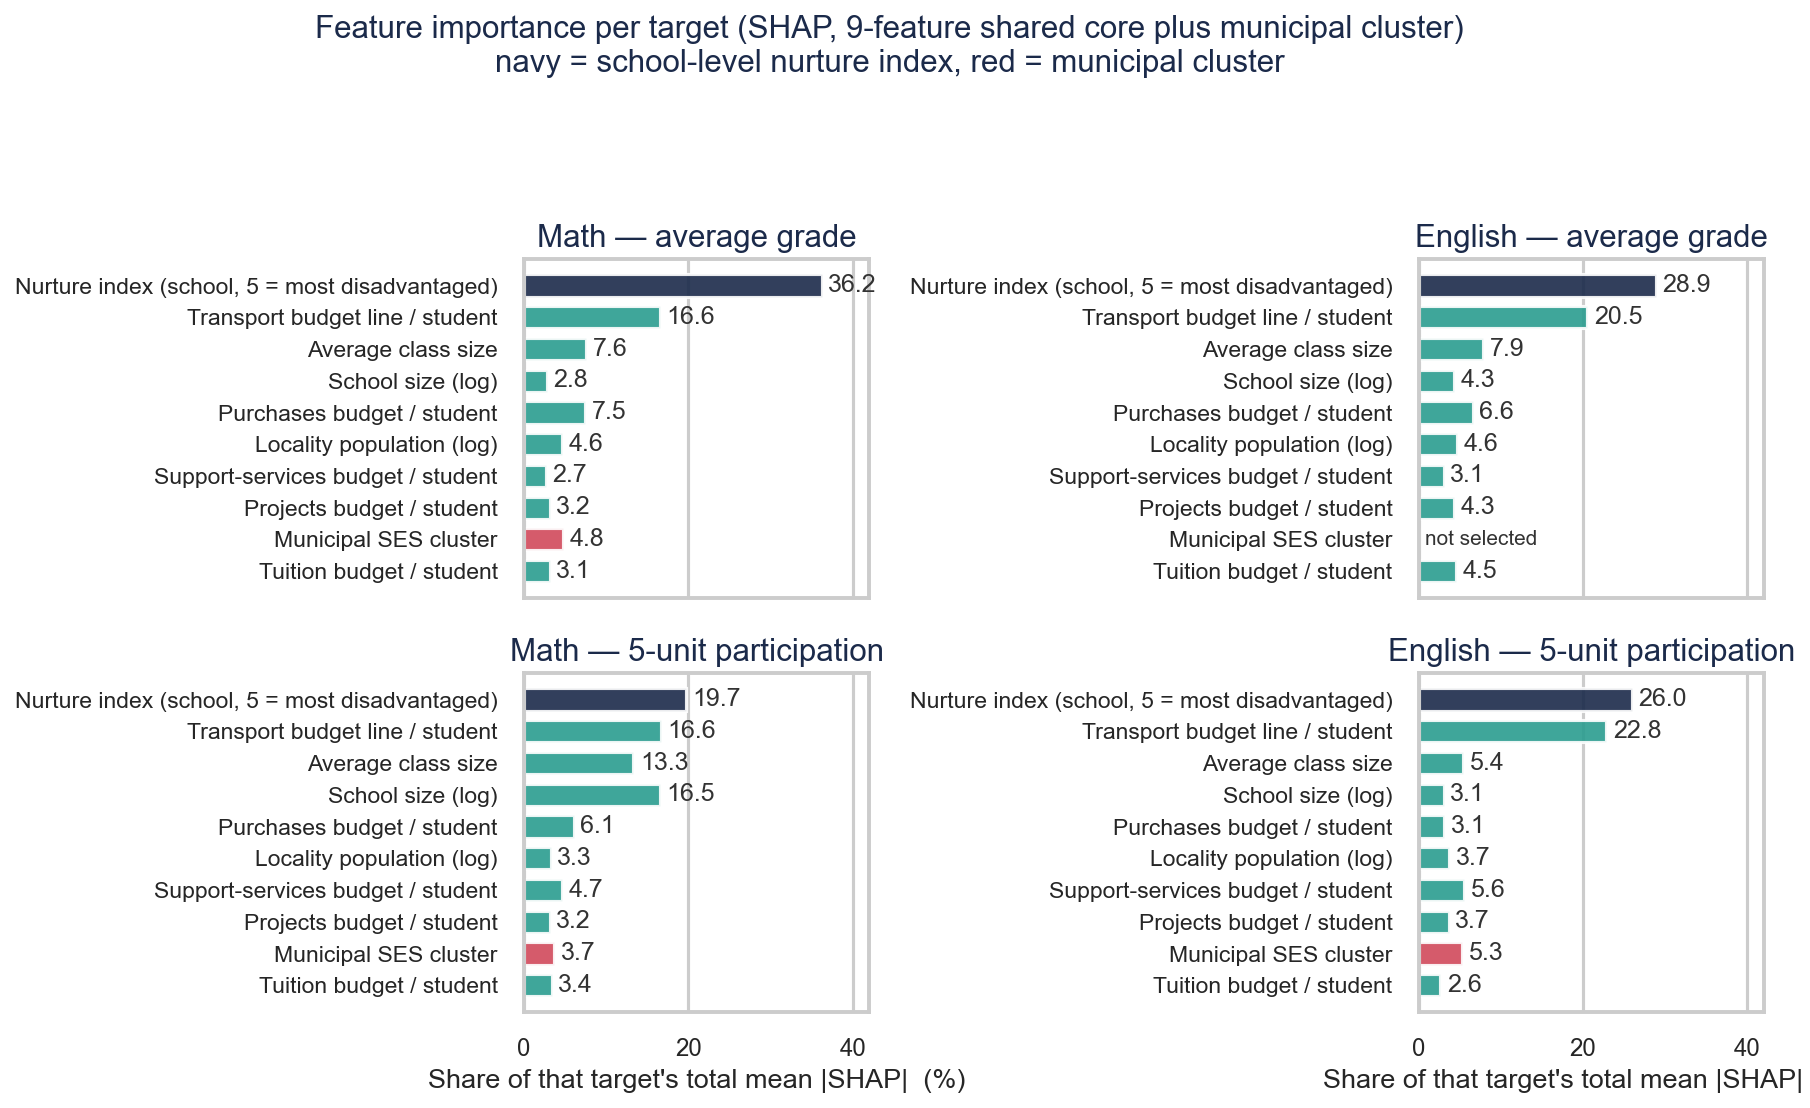
\includegraphics[width=0.92\linewidth]{section7/shap_core_ranking.png}
\caption{Mean $|$SHAP$|$ importance as a share of each target's total, from a
RandomForest refit matching the selected champion. The school-level nurture
index leads all four outcomes (19.7\% to 36.2\%), while municipal cluster never
exceeds 5.3\% and is not selected at all for English average grade.}
\label{fig:shap}
\end{figure}

\textbf{How much the school-level data adds.} SHAP ranks features inside a model
but cannot say what the extra data was worth. So each target is modelled twice on
\emph{identical rows} under the same nested protocol: once on municipal features
alone (cluster, population, locality type, year) and once on the full candidate
set. Only the available information differs, so the gap measures incremental
predictive value (Table~\ref{tab:ablation}).
\phantomsection\label{sec:secondary}

\begin{table}[H]
\centering
\footnotesize
\renewcommand{\arraystretch}{1.3}
\caption{Ablation study under the same nested protocol: outer-fold $R^2$
(mean $\pm$ sd) from municipal features alone, and the gain from adding the
school-level set on identical rows. The full-set scores are the Random Forest
column of Table~\ref{tab:leaderboard} and so are not repeated here.}
\label{tab:ablation}
\begin{tabular}{@{}>{\raggedright\arraybackslash}p{3.2cm}rccc@{}}
\toprule
\textbf{Target} & \textbf{Rows} & \textbf{Municipal only} & \textbf{$\Delta R^2$ from school data} & \textbf{Folds improved} \\
\midrule
Math grade              & 2,995 & $0.109\!\pm\!0.019$ & $\mathbf{+0.311\!\pm\!0.040}$ & 5/5 \\
English grade           & 2,963 & $0.196\!\pm\!0.028$ & $\mathbf{+0.256\!\pm\!0.034}$ & 5/5 \\
Math 5-unit             & 3,221 & $0.055\!\pm\!0.033$ & $\mathbf{+0.340\!\pm\!0.039}$ & 5/5 \\
English 5-unit          & 3,226 & $0.229\!\pm\!0.050$ & $\mathbf{+0.328\!\pm\!0.043}$ & 5/5 \\
\midrule
\textbf{Mean} & & \textbf{0.147} & $\mathbf{+0.309}$ & \textbf{20/20} \\
\bottomrule
\end{tabular}
\end{table}

Municipal features alone predict little, with advanced Math participation close
to unpredictable from the town. Adding the school-level set raises every target
to between 0.395 and 0.557, a mean gain of $+0.309$ holding in \textbf{every
outer fold}, so it is not an artefact of a favourable split. The result is
associational: incremental predictive value, not a causal effect of school
resources.

\textbf{Subject resilience and low-status overachievers.} The secondary questions
use the municipal gradient alone, holding institutional features out so they read
as a clean measure of socioeconomic disparity (Table~\ref{tab:secondary}).
Comparing cluster~2 against cluster~9, Mathematics is the more resilient subject:
a slightly smaller achievement gap and a participation gap roughly a third of
English's. Overachievers are clusters~1--4 schools whose average grade reaches
the \emph{median} of clusters~8--10 (84.90). Of 460 such schools, \textbf{87
(18.9\%)} clear that bar, and on Welch two-sample tests their advanced-track
participation is roughly 2.7$\times$ their peers' in Math and 2.6$\times$ in
English.

\begin{table}[H]
\centering
\footnotesize
\renewcommand{\arraystretch}{1.25}
\caption{Secondary questions. Resilience contrasts cluster~2 with cluster~9.
Overachievers are clusters~1--4 schools at or above the clusters~8--10 median
grade (84.90). The comparison group is the remaining low-cluster schools.}
\label{tab:secondary}
\begin{tabular}{@{}>{\raggedright\arraybackslash}p{5.0cm}rrr@{}}
\toprule
\textbf{(A) Resilience, cluster 2 $\rightarrow$ 9} & \textbf{Math} & \textbf{English} & \\
Grade gap (points), Cohen's $d$ & 6.18 (0.91) & 6.45 (1.16) & \\
5-unit participation gap & \textbf{0.115} & 0.367 & \\
\midrule
\textbf{(B) Overachievers, 87 of 460} & \textbf{Over} & \textbf{Peers} & \textbf{$p$} \\
Math 5-unit participation & 0.132 & 0.049 & $1.4\!\times\!10^{-5}$ \\
English 5-unit participation & 0.468 & 0.181 & $1.4\!\times\!10^{-11}$ \\
\bottomrule
\end{tabular}
\end{table}

\section{Results and Conclusions}
\label{sec:conclusions}

\textbf{Main question.} Combined, municipal socioeconomics and school-level
resources predict Bagrut outcomes usefully: nested out-of-fold $R^2$ of 0.40 to
0.56 (Table~\ref{tab:leaderboard}) with near-zero mean residuals
(Figure~\ref{fig:residuals}). \emph{Combined} carries it: municipal data alone
reaches only 0.06 to 0.23, and the school-level features lift every target by
$+0.309$ on average, in every outer fold (Table~\ref{tab:ablation}).

\textbf{Secondary question A.} Mathematics is the more resilient subject
(Table~\ref{tab:secondary}): the cluster~2 to cluster~9 gap is smaller for Math
in achievement and about a third of English's in participation. Overachieving
schools clearly exist, 87 of 460 low-cluster schools, with significantly higher
advanced-track participation than their peers.

\textbf{Secondary question B.} The strongest school-level predictor is the
Ministry's per-school nurture index, first for all four targets, followed by the
transport-related budget field, school size, and class size. Five per-student
budget ratios are confirmed for every target (Section~\ref{sec:importance}).
Municipal cluster never exceeds 5.3\% of attribution and is dropped for English
average grade.

\textbf{Conclusion.} Socioeconomic status matters, but the municipal average is
much coarser than the school-level measure. Measured per school the same
construct dominates every model. The town-level cluster is among the weakest
features retained and is rejected entirely for one target.

\textbf{Limitations and further work.} The institutional data is a single 2014/15
snapshot applied to all four exam years, so within-school change cannot be
separated. Suppressed grade cells are small cohorts, so the smallest schools are
underrepresented, and complete-case modelling removes a further 9--12.5\% of
rows. The transport field's negative values leave its meaning unconfirmed.
Results are associational, and this model is not suitable for individual
admissions decisions or for withholding resources from schools. Natural
extensions: per-year budget records to test whether spending \emph{precedes}
outcomes, a study of the 87 overachievers, and bounded-response models for
participation rates.


\begingroup
\footnotesize
\setlength{\parskip}{0pt}
\begin{thebibliography}{9}
\setlength{\itemsep}{0pt}
\setlength{\parsep}{0pt}
\bibitem{bagrut} Israel Ministry of Education. \emph{Bagrut examination results
  by school, 2013--2016}. Freedom of Information Law, mirrored on Kaggle.
\bibitem{cbs} Israel Central Bureau of Statistics. \emph{Characterization and
  Classification of Local Authorities by Socio-Economic Level}, 2015 index.
\bibitem{moe} Israel Ministry of Education. \emph{Institutional budget and
  school characteristics file}, 2014/15.
\bibitem{mice} van Buuren, S. and Groothuis-Oudshoorn, K. (2011). mice:
  Multivariate Imputation by Chained Equations in R. \emph{J.\ Stat.\ Soft.}, 45(3).
\bibitem{boruta} Kursa, M. B. and Rudnicki, W. R. (2010). Feature Selection with
  the Boruta Package. \emph{J.\ Stat.\ Soft.}, 36(11).
\bibitem{shap} Lundberg, S. M. and Lee, S.-I. (2017). A Unified Approach to
  Interpreting Model Predictions. \emph{NeurIPS 30}.
\bibitem{iforest} Liu, F. T., Ting, K. M. and Zhou, Z.-H. (2008). Isolation
  Forest. \emph{IEEE ICDM}, 413--422.
\bibitem{lof} Breunig, M. M. et al. (2000). LOF: Identifying Density-Based Local
  Outliers. \emph{ACM SIGMOD}, 93--104.
\bibitem{sklearn} Pedregosa, F. et al. (2011). Scikit-learn: Machine Learning in
  Python. \emph{JMLR}, 12, 2825--2830.
\end{thebibliography}
\endgroup

\end{document}
